\documentclass[tesis.tex]{subfiles}

\begin{document}
	
\chapter{Grafos de Cayley.} \label{seccion_treewidth}

Las referencias centrales de este capítulo son \cite{diekert2017context}, \cite{kuske2005logical} y \cite{diestel2005graph}.

En la primer sección \ref{} introducimos las descomposiciones en árboles para grafos no dirigidos y así la definición de treewidth.
La construcción del ejemplo \ref{} es de vital para probar el teorema de Muller--Schupp.

En la segundo sección \ref{} introducimos brevemente las ideas centrales detrás de las cuasisometrías (en nuestro caso restringidas al contexto de grafos pero bien podría ser para cualquier espacio métrico en general).
La idea es poder usar estas herramientas para probar que todo grafo de Cayley de un grupo \fg tiene treewidth finito, es decir que no depende de los generadores.

Finalmente en la sección \ref{} probamos uno de los resultados centrales que nos dice que todo grupo independiente de contexto tiene treewidth finito.
Este es el teorema central del trabajo \cite{} aunque en nuestro caso lo reescribimos para en vez de trabajar con triangulaciones de grafos usemos el treewidth.



\section{Treewidth.}

Dado que el grafo de Cayley de todo grupo libre se puede tomar para que sea un árbol es razonable pensar que todo grupo virtualmente libre es tal que su grafo de Cayley se parezca a un árbol. 
Vamos a dar una primera definición que nos permite formalizar esta idea de que un grafo se parezca a un árbol.
Esta definición es la del treewidth, noción originalmente introducida por .... en \ref{}.

\begin{deff}\label{desc-arbol}
	Una \emph{descomposición en un árbol} de un grafo $\Gamma$ es un par $(T,f)$ donde
	$T$ es un árbol y $f$ un mapa 
	\[
	f: V(T) \to 2^{V(\Gamma)}
	\]
	Que cumple las siguientes condiciones:
	\begin{enumerate}
		\item[\textbf{T1.}] Para todo vértice $v \in V(\Gamma)$ debe existir $t \in V(T)$ tal que $v \in f(t)$. 
		\item[\textbf{T2.}] Para toda arista $\{v,w\} \in E(\Gamma)$ 
		debe existir $t \in V(T)$ tal que $v,w \in f(t)$.
		\item[\textbf{T3.}] Si $v \in V(\Gamma)$ es tal que $v \in f(t) \cap f(s)$ luego $v \in f(r)$ para todo $r \in V(T)$ en la geodésica que va desde $s$ a $t$ dentro de $T$.  
	\end{enumerate} 
\end{deff}
Notemos que la tercer condición \textbf{T3} se puede reescribir de la siguiente manera:
dado $v \in V(\Gamma)$ entonces el conjunto $\{ t \in V(T) :  v \in f(t) \}$ forma un subárbol de $T$.

Dado $t \in V(T)$ llamaremos a $f(t) \in 2^{V(\Gamma)}$ un \emph{bolsón}.

\begin{center}
	\missingfigure[figwidth=6cm]{Mostrar como son los bolsones.}
\end{center}

\smallskip
Si queremos que una descomposición en un árbol de un grafo nos modelice la idea que el grafo se parece a un árbol entonces nos va a interesar que los \emph{bolsones} $f(t) \in 2^{V(\Gamma)}$ no tengan muchos vértices. 
Esto nos conduce a la siguiente definición.

\begin{deff}
	Dado un grafo $\Gamma$ y $(T,f)$ una descomposición en un árbol de $\Gamma$ el \emph{bagsize} de esta descomposición es el siguiente valor:
	\begin{equation*}
		bs(X,T,f) = \sup_{t \in V(T)} |f(t)| - 1
	\end{equation*}
	Un grafo $X$ tiene \emph{treewidth finito} si existe una descomposición en un árbol de bagsize finito.	
\end{deff}

Probemos con esta definición que sucede lo que es razonable que suceda.
Esto es que dado $T$ un árbol vale que $T$ tiene treewidth finito y más aún el bagsize de $T$ se puede tomar para que sea exactamente $1$.

\begin{deff}
	Dado $\Gamma$ un grafo no dirigido llamaremos a $\Gamma'$ \emph{la subdivisión baricéntrica de $\Gamma$ }al grafo no dirigido dado por
	$V(X') = V(X) \cup E(X)$ y $E(X') = \{ \{ v, \{v,w \} \} \mid \ \text{si} \ \{ v,w \} \in E(\Gamma) \}$.
\end{deff}

Gráficamente lo representamos de la siguiente manera:
\begin{center}
	\missingfigure[figwidth=6cm]
	{Dibujo de subdivisión baricéntrica}
\end{center}

\begin{obs}\label{obs_sub_bari_arbol}
	Si $T$ es un árbol entonces la subdivisión baricéntrica de $T$ también es un árbol.
\end{obs}

\begin{ej}\label{desc-arbol-arbol}
	Sea $T$ un árbol probemos que $T$ tiene treewidth exactamente igual a $1$.
	
	Para eso consideremos el siguiente par $(T',f)$ donde $T'$ es la subdivisión baricéntrica de $T$ y por lo tanto es un árbol por \ref{obs_sub_bari_arbol} y donde $f$ está definida como
	\[
	f(t) = 
	\begin{cases}
		\{ v \} \ & \text{si} \ t = v \in V(T) 				\\
		\{ v,w  \} \ &\text{si} \ t = \{ v,w\} \in E(T).
	\end{cases}
	\]
	
	
	Por como definimos a $f$ es evidente que $|f(t)| \le 2$ para todo $t \in V(T)$.
	De esta manera si vemos que $(T',f)$ se trata de una descomposición en un árbol para $T$ tendremos probado que $bs(T,T',f) = 1$ tal como queríamos ver.
	
	Finalmente lo único que nos queda por probar es que se trata de una descomposición en un árbol.
	Esto es que cumple las tres condiciones necesarias.
	\begin{enumerate}
		\item[\textbf{T1.}] 
		Sea $t \in V(T)$ luego consideremos $f(t) = \{ t \}$ dado que $t \in V(T')$ por construcción de la subdivisión baricéntrica.
		
		\item[\textbf{T2.}] 
		Dada una arista $\{t,s\} \in E(T)$ consideramos $f(\{ t,s \}) = \{ t,s \} $ de manera que tanto $t$ como $s$ están en un mismo bolsón.
		
		\item[\textbf{T3.}] 
		Sea $t \in V(T)$, queremos ver que $\{ t' \in V(T') :  t \in f(t') \}$ resulta ser un subárbol de $T'$.		
		Para empezar tenemos que $t \in f(t')$ si y solo sí sucede alguno de dos casos:
		$t' = t$ o bien ocurre que $t' = \{ t,s \}$ para cierta arista $\{t,s\} \in E(T)$.
		En particular notemos que todos estos vértices de $T'$ están conectados y en particular son un subgrafo dado que $ \{t, \{t,s\}\} \in E(T')$ para $t \in V(T)$ y $\{t,s\} \in E(T)$. 
	\end{enumerate}
	
	
\end{ej}

Probaremos algunas proposiciones útiles de las descomposiciones en árboles de grafos.
Esta primer proposición generaliza la propiedad \textbf{T3} de una descomposición.
Sean $t,s \in V(T)$ vértices cualesquiera entonces existe una única geodésica que las une. 
Denotemosla $[t,s]$.
\todo{Mencionar 1- árboles uni geod 2- concatenacion de caminos} 
\begin{prop}\label{prop-camino-desc}
	Sea $\Gamma$ grafo no dirigido.
	Sea $(T,f)$ una descomposición en un árbol de $\Gamma$.
	Sean $t_{1},t_{2},t_{3} \in V(T)$ tales que $[t_1,t_2]$ pasa por $t_{3}$.
	Sean $v,w \in V(\Gamma)$ de manera que $v \in f(t_{1})$ y tal que $w \in f(t_{2})$.
	Si $\gamma = v_0 \dots v_n$ es algún camino en $\Gamma$ conectándolos de manera que $v_{0}=v$ y $v_{n} = w$	
	entonces debe existir algún $ 0 \le i \le n$ de manera que $v_i \in f(t_{3})$. 
\end{prop}

\begin{proof}	
	Vamos a demostrarlo haciendo inducción en la longitud $|\gamma|$.
	 
	El caso base es que $|\gamma| = 0$ por lo tanto $v=w$. 
	En este caso por ser $(T,f)$ una descomposición en un árbol tenemos que usando \textbf{T3} vale que $\{  t \in V(T) \mid v \in f(t) \}$ es un subárbol, por lo que $v \in f(t_{3})$.
	
	Para el paso inductivo supongamos que vale para caminos de longitud $n$.
	Sea $t' \in V(T)$ de manera que $v_{0}, v_{1} \in f(t')$ que existe por la propiedad \textbf{T2}.
	Dado que 
	$[t_{1}, t_{2}] = [t_{1}, t']*[t',t_{2}]$
	luego $t_{3}$ está en alguna de las dos geodésicas: $[t_{1},t']$ o $[t',t_{2}]$.
	
	Si $t_{3}$ está en la primera geodésica entonces $t' = t_{3}$ y ya está porque nos alcanza con tomar $i=1$ de manera que $v_1 \in f(t_{3})$.
	En el otro caso consideramos el camino de longitud $n$ dado por $(v_1 v_2 \dots v_n)$ y usando la hipótesis inductiva llegamos al resultado.	
\end{proof}

\begin{prop}\label{prop_tw_finitos_bolsones}
	Sea $\Gamma$ un grafo localmente finito con treewidth finito entonces podemos tomar una descomposición en un árbol $(T',f')$ de $\Gamma$ de manera que para todo $v \in V(\Gamma)$ valga que:
	\[
	| \{  t' \in V(T') : \ v \in f'(t)  \} | < \infty.
	\]
\end{prop}
\begin{proof}
	Sea $(T,f)$ una descomposición en un árbol de $\Gamma$ tal que tiene bagsize finito.
	Por la propiedad \textbf{T2} tenemos que para cada arista 
	$\{u,v\} \in E(\Gamma)$ existe al menos un vértice $t_{uv} \in V(T)$ de manera que $u,v \in f(t_{uv})$.
	
	Fijamos $v \in V(\Gamma)$ un vértice  de $\Gamma$.
	Consideremos el siguiente conjunto de vértices de $T$
	\[
		\{  t_{uv} \in V(T) \mid \exists v \in V(\Gamma), \ \{ u,v \} \in E(\Gamma)  \}.
	\]
	Notemos que es un conjunto finito porque por hipótesis $\Gamma$ es un grafo localmente finito.
	Sea $T'$ el subárbol finito de $T$ generado a partir de estos finitos vértices.
	
	Vamos a definir a $f'$ utilizando a $f$ de la siguiente manera
	
	\[
	f'(t) = 
	\begin{cases}
		f(t)  \ \  &\text{si} \ \  t \in V(T') \\
		f(t) \setminus \{  v \} \ \  &\text{si} \ \  t \notin V(T')
	\end{cases}
	\]
	haciendo esto mismo para cada uno de los vértices del grafo $\Gamma$ terminamos de definir a $(T',f')$.
	
	Finalmente chequeamos que sea trata de una descomposición en un árbol.
	Las primeras dos condiciones \textbf{T1} y \textbf{T2} se siguen cumpliendo porque por nuestra construcción de $T'$ garantizamos que se sigan cumpliendo.
	La condición \textbf{T3} es válida porque si tomamos $v \in V(\Gamma)$ por nuestra construcción el subgrafo 
	\[
		\{ t' \in V(T') \mid v \in f'(t') \}
	\]	
	es un subárbol generado a partir de una cantidad finita de vértices.
	Con esto probamos que $(T',f')$ es una descomposición en un árbol y como $|f'(t)| \le |f(t)|$ para todo $t \in V(T)$ luego obtenemos que el bagsize de $(T',f')$ también es finito.
\end{proof}

\begin{deff}
	Sea $\Gamma$ un grafo y $C \subseteq V(\Gamma)$ un conjunto de vértices entonces definimos los \emph{vecinos de $C$} por medio de 
	\[
	N(C) = \{ v \in V(\Gamma) \mid \exists w \in C, \ \{v,w \} \in E(\Gamma) \}.
	\]
	De esta manera podemos definir recursivamente los \emph{l-ésimos vecinos} por medio de $N^l(C) = N(N^{l-1}(C))$.
\end{deff}


	Si al grafo no dirigido $\Gamma$ lo interpretamos como un espacio métrico entonces podemos escribir esta definición de la siguiente manera un poco más concisa:
	\[
		N^l (C) = \{ v \in V(\Gamma) : \ \exists w \in C, \  d(v,w) \le l  \}
	\]
	Veamos ahora que dada una descomposición en un árbol si tomamos los vecinos de los bolsones podemos armarnos otra descomposición en un árbol.


\begin{prop}\label{prop-vecinos-desc}
	Sea $\Gamma$ un grafo no dirigido y sea $(T,f)$ una descomposición en un árbol para $\Gamma$.
	Dado $l \in \NN$ consideramos $(T,g)$ tal que $g(t) = N^l(f(t))$ entonces $(T,g)$ resulta ser una descomposición en un árbol para $\Gamma$.
\end{prop}
\begin{proof}
	Probemos este resultado haciendo inducción en $l$.
	
	Consideremos el caso base $l=1$.
	En este caso, las dos primeras condiciones de la descomposición en un árbol \textbf{T1} y \textbf{T2} se siguen cumpliendo porque no hicimos más que agrandar los bolsones. 
	Esto es que $f(t) \subseteq g(t)$.
	
	Debemos ver que $(T,g)$ cumple \textbf{T3}.
	Queremos ver que si fijamos $v \in V(\Gamma)$ el conjunto 
	\[
		T_{v} = \{ t \in V(T) \mid v \in g(t)  \}
	\]
	forma un subárbol de $T$. 
	Para ver esto nos basta con ver que $T_{v}$ es conexo.
	Como los árboles son únicamente geodésicos podemos ver equivalentemente lo siguiente:
	dados $t_{1}, t_{2} \in T_{v}$ entonces para todo $t_{3}$ que esté en la geodésica $[t_{1}, t_{2}]$ vale que $t_{3} \in T_{v}$. 
	
	Como $v \in g(t_{1})$ entonces existe $w \in f(t_{1})$ adyacente (o bien podría ser exactamente $v$) a $v$.
	Similamente existe $u \in f(t_{2})$ adyacente (o bien podría ser exactamente $v$) a $v$.
	
	Consideramos el camino de tres vértices $\gamma = (w,v,u)$ y usamos la proposición \ref{prop-camino-desc} para concluir que, sin pérdida de generalidad, $v \in f(t_{3})$.
	De esta manera vemos que necesariamente $v \in g(t_{3})$ tal como queríamos ver.
		
	El paso inductivo se sigue directamente del caso base.
	Esto se debe a que si sabemos que $(T,g)$ con $g(t) = N^{l-1}(f(t))$ forma una descomposición de un árbol entonces podemos usar el caso base para ver que los vecinos de esta descomposición siguen siendo otra descomposición en un árbol y con esto terminamos de probarlo porque $N^l(f(t)) = N (N^{l-1})(f(t))$.
\end{proof}
\medskip

\begin{deff}
	Dado un grafo $\Gamma$ y un conjunto de vértices $C \subseteq V(\Gamma)$ definimos el \emph{borde de vértices} de $C$ como:
	\[
	\beta C =  N(C) \cap N(\ol{ C})
	\] 
	por otro lado tenemos que el \emph{borde de aristas} de $C \subseteq V(\Gamma)$ se define como:	
	\[
	\delta C = \{  \{v,w \} \in E(\Gamma) \mid v \in C, w \in \ol C    \}.
	\]
\end{deff}


\begin{center}
	\missingfigure[figwidth=6cm]{Dibujo ilustrativo.}
\end{center}

\begin{ej}\label{desc-grafo-cayley}%[Descomposición válida para todo grupo finitamente generado].
	
	Construyamos una descomposición en un árbol que podemos hacer en general para todos los grafos de Cayley de grupos finitamente generados. 
	Consideremos el grafo $\Gamma = \text{Cay}(G,A)$ para cierto conjunto de generadores $A$ finito.
		
	
	Sea $V_l = \Gamma \setminus N^l(\{1\}) $ tal que $V_0 = \Gamma \setminus \{1\}$. 
	Los vértices del árbol $T$ van a estar dados por los siguientes conjuntos:
	\[
	V(T) = \{  \beta C : \exists l \in \NN / C \subseteq V_l \ \text{componente conexa} \} \cup \{ 1 \}
	\]
	estamos tomando todos los posibles bordes de vértices 
	de todas las componentes conexas de todos los $V_l$ con $l \in \NN$.
	 
	Antes de definir las aristas notemos lo siguiente.
	Si $C$ es una componente conexa de $V_{l+1}$ entonces tiene que existir $D$ componente conexa de $V_{l}$ de manera tal que $C \subseteq D$.
	Esto se debe a que $V_{l+1} \subseteq V_{l}$ y a su vez como $C$ es conexo si interseca a una componente conexa necesariamente tiene que estar incluido en esta componente.
	Las aristas van a estar dadas por lo siguiente:
	\[
	E(T) = \{ \{ \beta C, \beta D \} : \exists l \in \NN / \ C \subseteq D \subseteq V_l \land \ C \subset V_{l+1}  \} \cup \{  \{1,\beta C\} : C \subseteq V_0  \}
	\]
	
	Probemos que el grafo $T$ resulta ser un árbol. 
	
	\begin{enumerate}[$\bullet$]
		\item \textbf{$T$ es conexo.}
		Probaremos la siguiente afirmación que va a implicar la conectividad de $T$:
		Para todo $\beta C \in V(T)$ existe un camino que lo conecte con $1$.
		Lo probaremos por inducción en $l$ siendo $l \in \NN$ tal que $C$ es una componente conexa de $V_{l}$.
		
		El caso base es $l = 0$ y en este caso tenemos que $\{ 1, \beta C  \}$ para todo $C \in V_{0}$ por definición de las aristas de $T$.
		
		Para el paso inductivo suponemos que todo $\beta D$ para $D$ componente conexa de $V_{l}$ está conectado con $1$.
		Sea entonces $C$ componente conexa de $V_{l+1}$, notemos que necesariamente tiene que existir $D$ componente conexa de $V_{l}$ tal que $C \subseteq D$ dado que $C$ es conexo y $V_{l+1} \subseteq V_{l}$.
		
		\item \textbf{$T$ es acíclico.}
		Probemos que todo camino cerrado en $T$ no es simple.
		Para eso sea $\gamma$ un camino cerrado (no constante sino no hay nada que probar) en $T$ tal que empieza y termina en $\beta E$ donde $E$ es alguna componente conexa para algún $V_{k}$.
		Sea $C$ tal que $\beta C$ es uno de los vértices del camino $\gamma$ y es componente conexa de $V_{l}$ con $l$ maximal en el camino.
		Supongamos sin pérdida de generalidad que $E$ es distinto de $C$ porque sino podemos modificar el comienzo y final del camino porque es un camino cerrado.
		Necesariamente tenemos que si $\{ \beta D, \beta C \}$ es una arista del camino entonces $D$ es componente conexa de $V_{l-1}$.
		Esto nos dice que el camino $\gamma$ tiene la siguiente pinta
		\[
			\gamma = (\beta E, \dots, \beta D, \beta C, \beta D, \dots, \beta E)
		\]
		por lo que el camino no es simple dado que tiene dos veces a la misma arista $\{ \beta C, \beta D \}$.
		
	\end{enumerate}
	  
	Sea entonces $f: V(T) \to 2^{V(\Gamma)}$ la función definida por $f(\beta C) = \beta C$ donde en el lado izquierdo lo miramos como un vértice y en el lado derecho como un conjunto de vértices de $\Gamma$.
	Afirmamos que $(T,f)$ es una descomposición en un árbol para el grafo de Cayley $\Gamma$.
	Para verlo debemos ver que cumple las tres condiciones \ref{desc-arbol} de la definición. 
	\begin{enumerate}
		\item[\textbf{T1.}] Sea $g \in V(\Gamma)$ luego si $d(1,g) = l$
		tenemos que $g \in C \subseteq V_{l-1}$ para cierta $C$ componente conexa de $V_{l-1}$ y en particular $g \in \beta C$.		 
		
		
		\item[\textbf{T2.}] Sea una arista $\{g,h\} \in E(\Gamma)$ 
		Separamos en dos casos dependiendo si $d(g,1) = d(h,1)$ o si no sucede esto.
		
		Supongamos que ambas están a la misma distancia del vértice $1$. 
		En tal caso sea $l$ tal que 
		\[
			d(g,1)= l = d(h,1)
		\] 
		luego tiene que existir $C$ componente conexa de $V_{l-1}$ 
		tal que $g,h \in C$ dado que ambos vértices están conectados.
		Tenemos en particular que $g,h \in \beta C$.
		
		
		El otro caso es que las distancias al vértice $1$ son distintas aunque necesariamente están restringidas a que sean del tipo
		\[
			d(g,1)= l < l+1 = d(h,1)
		\] 
		y en este caso como $g,h$ están conectados resulta que $g,h \in \beta C$ si $C$ es la componente conexa que contiene a $h$ en $V_l$.
		
		\item[\textbf{T3.}] Queremos ver que si fijamos $g \in V(\Gamma)$ entonces el subgrafo $T_{g} = \{ t \in V(T) \mid g \in f(t) \} $ es un subárbol de $T$.
		Para eso notemos que si $d(g,1) = l$ luego
		existe una única componente conexa $D \in V_{l-1}$ de manera que $g \in \beta D$ y como el grafo de Cayley de un grupo \fg es localmente finito entonces existen finitas componentes conexas $C_{1}, \dots, C_{k}$ de $V_{l}$ de manera que $g \in \beta C_{1}, \dots, g \in \beta C_{k}$.
		Notemos que $T_{g}$ es conexo porque para todo $\beta C_{i}$ vale que $\{ \beta D, \beta C_{i} \} \in E(T)$ por lo que $T_{g}$ resulta ser un subárbol de $T$ tal como queríamos ver.
		 
		
	\end{enumerate}
\end{ej}

\section{Cuasisometrías.}

Nuestro objetivo es introducir las cuasisometrías para garantizar que la propiedad de tener treewidth finito no dependa de los generadores elegidos.
Esta subsección sigue los textos de \cite{bridson2013metric} y de \cite{loh2017geometric}.

\begin{deff}
	Sean $(X,d_X),(Y,d_Y)$ espacios métricos. 
	Una \emph{cuasisometría} es una función $f:X \to Y$ tal que:
	\begin{itemize}
		\item[\textbf{Q1.}] Existe constante $A > 0$ tal que para todo par de puntos $x_1,x_2 \in X$ hace valer la siguientes desigualdades
		\[
		\frac{1}{A} d_X(x_1,x_2) - A \le d_Y(f(x_1),f(x_2)) \le A d_X(x_1,x_2) + A
		\]
		\item[\textbf{Q2.}] Existe una constante $C \ge 0$ tal que para todo punto $y \in Y$ debe existir $x \in X$ de manera que 
		\[
		d(y,f(x)) \le C
		\]
	\end{itemize}
\end{deff}

Intuitivamente una cuasisometría entre espacios métricos nos dice que estos resultan ser globalmente similares y las diferencias que tienen localmente están uniformemente acotadas. 
\medskip
\begin{prop}\label{prop_qi_simetrica}
	Si existe $f:X \to Y$ cuasisometría entonces también debe existir $g:Y \to X$ cuasisometría y constantes positivas $C,D \in \RR$ tal que:
	\begin{itemize}
		\item $d(g \circ f (x), x) < C$ para todo $x \in X$.
		\item $d(f \circ g (y), y) < D$ para todo $y \in Y$. 
	\end{itemize}
\end{prop}
\begin{proof}
	Ver \cite{loh2017geometric}.
\end{proof}

\begin{deff}
	Dos espacios métricos que se dicen \emph{cuasisométricos} si existe una cuasisometría entre ellos.
\end{deff}

Vale el siguiente resultado que se desprende de la proposición \ref{prop_qi_simetrica}.
\begin{prop}
	Ser cuasisométricos es una relación de equivalencia entre espacios métricos.
\end{prop}
\begin{proof}
	Ver \cite{loh2017geometric}.
\end{proof}

En nuestro caso en particular los espacios métricos que nos van a interesar son los grafos no dirigidos.
Más aún nos vamos a interesar en los grafos de Cayley de grupos finitamente generados.

El siguiente resultado que enunciamos sin demostración nos garantiza que todos los grafos de Cayley para un grupo finitamente generado son cuasisométricos entre sí.
\begin{prop}
	Sea $G$ grupo finitamente generado por $\Sigma$ y por $\Delta$, ambos conjuntos finitos entonces $\text{Cay}(G,\Sigma)$ y $\text{Cay}(G, \Delta)$ son cuasisométricos entre sí.
\end{prop}

\begin{proof}
	Resultado estándar. 
	Ver \cite{bridson2013metric}.
\end{proof}

Este resultado deja de ser cierto en el contexto que tomamos un conjunto de generadores que no es finito.

Para probar que alguna propiedad que depende de los grafos de Cayley es invariante por generadores nos alcanza con ver que esta propiedad es invariante por cuasisometrías.
En nuestro caso en particular veamos que el treewidth es un invariante por cuasisometría y entonces no depende de los generadores elegidos y por lo tanto es una propiedad intrínseca del grupo. 

\begin{prop} \label{treewidth-inv}
	Sean $(\Gamma_{1},d_{1}), (\Gamma_{2}, d_{2})$ grafos no dirigidos vistos como espacios métricos tales que $\Gamma_{1}$ tiene treewidth finito.
	Sea $\phi:(\Gamma_{1},d_{1})\to (\Gamma_{2},d_{2})$ una cuasisometría.
	Entonces $\Gamma_{2}$ tiene treewidth finito.
\end{prop}

\begin{proof}
	Sea la cuasisometría $\phi$ tal que existe una constante $A > 0$ de manera que para todo par $v_{1}, v_{2} \in \Gamma_{1}$ tenemos que
	\[
	\frac{1}{A} d_X(v_1,v_2) - A \le d_Y(\phi(v_1),\phi(v_2)) \le A d_X(v_1,v_2) + A
	\]
	y existe una constante $C \ge 0$ tal que para todo $w \in \Gamma_{2}$ debe existir $v \in \Gamma_{1}$ de manera que
	\[
	d(w,\phi(v)) \le C.
	\]
	
	Sea $(T,f)$ una descomposición en un árbol para $\Gamma_{1}$ tal que tiene bagsize finito.
	Si consideramos a $g: V(T) \ni t \mapsto N^{A(2C+1)}(f(t)) \in 2^{V(\Gamma_{1})}$ luego $(T,g)$ es una descomposición en un árbol para $\Gamma_{1}$ por el lema \ref{prop-vecinos-desc}.
	Consideremos entonces la siguiente función 
	\[
		h: V(T) \ni t \mapsto N^{C+1}(\phi(g(t))) \in 2^{V(\Gamma_{2})}
	\]
	afirmamos que $(T,h)$ es una descomposición en un árbol para $\Gamma_{2}$ tal que tiene bagsize finito.
	
	
	Para ver esto debemos ver que cumple las tres condiciones que definen a una descomposición en un árbol.
	\begin{enumerate}[T1.]
		\item Sea $w \in V(\Gamma_{2})$ luego por la definición de cuasisometría existe $v \in V(\Gamma_{1})$ tal que $d(w, \phi(v)) \le C$.
		En particular tenemos que si $w \in g(t)$ para $t \in V(T)$ luego  $w \in N^l(\phi(g(t))) = h(t)$ tal como queríamos ver.
		
		\item Sea $\{w,w'\} \in E(\Gamma_{2})$ luego si $v \in V(\Gamma_{1})$ es tal que $d(\phi(v),w) \le C$ entonces $d(\phi(v),w') \le C+1$.
		Esto nos dice que si $v \in g(t)$ luego $w,w' \in h(t)$ tal como queríamos ver.
		
		\item Veamos que el conjunto 
		\[
			T_{w} = \{ t \in V(T) \mid w \in h(t)   \}
		\]
		es un subárbol de $T$.
		Para esto vamos a ver que si $w \in h(t)$ y $w \in h(s)$ entonces existe $r \in V(T)$ tal que 
	\end{enumerate}
	
\end{proof}




%\begin{proof}
%	Si tenemos una cuasisometría $f:\Gamma_1 \to \Gamma_2$ tal que $\Gamma_2$ tiene treewidth finito $k \in \NN$, nos gustaría ver que $\Gamma_1$ también tiene esta propiedad.
%	Consideremos $l$ tal que $d(f(v),f(w)) \le l$ para vértices $v,w \in V(\Gamma_1)$ que estén conectados por una arista.
%	Esto lo podemos tomar porque al ser una cuasisometría 
%	\[
%	d(f(v),f(w)) \le C d(v,w) + C  \le 2C
%	\]
%	entonces basta con tomar $l \ge C+1$.
%	
%	Veamos de armarnos la descomposición en un árbol $T$ para $\Gamma_1$.	
%	Tomaremos como árbol para descomposición al mismo $T$ que usamos para $\Gamma_2$.
%	Sean $X(t)$ los bolsones de esta descomposición. 
%	Recordemos que por \ref{prop-vecinos-desc} si tomamos $N^l(X(t))$ los vecinos del bolsón $X(t)$ que están a distancia no mayor a $l$ seguimos teniendo una descomposición.  
%	Consideraremos los bolsones $Y(t) = f^{-1}(N^l(X(t)))$ de vértices en $\Gamma_1$. 
%	
%	Debemos ver que cumplen las tres propiedades.
%	
%	\begin{enumerate}
%		\item[\textbf{T1.}] La primera se cumple puesto que los bolsones $X(t)$ cubren $V(\Gamma_2)$. 
%		De esta manera $\bigcup_{t \in T} N^l(X(t)) = V(\Gamma_2)$ y por lo tanto tomando preimagen tenemos que
%		\[
%		\bigcup_{t \in V(T)} f^{-1} (N^l (X(t))) = \bigcup_{t \in V(T)} Y(t) = f^{-1} (V(\Gamma_2)) = V(\Gamma_1)
%		\] 
%		donde usamos que la preimagen de la unión es la unión de las preimágenes.
%		\item[\textbf{T2.}] La segunda condición usamos que si hay una arista $xy \in E(\Gamma_2)$ luego debe ser que $d(f(x),f(y)) \le l$ por como tomamos a $l$.
%		De esta manera como $f(x) \in X(t)$ para algún $t \in V(T)$, notemos que $f(y) \in N^l(X(t))$ también. 
%		Tomando preimagen tenemos que $x,y \in f^{-1}(N^l(X(t)))$ y esto es que justamente $x,y \in Y(t)$ para un mismo $t \in V(T)$ tal como queríamos ver.		
%		\item[\textbf{T3.}] Para la tercera condición si $x \in Y(t) \cap Y(s)$ queremos ver que $x \in Y(r)$ para todo $r \in V(T)$ que aparezca en la geodésica de $s$ a $t$.
%		Como la preimagen de una intersección es lo mismo que la intersección de las preimágenes entonces 
%		\[
%		x \in f^{-1}(N^l(X(t))) \cap f^{-1}(N^l(X(s))) = f^{-1}(N^l(X(t)) \cap N^l (X(s))
%		\]
%		de esta manera debe existir $v \in V(\Gamma_2)$ tal que $v \in N^l(X(s)) \cap N^l(X(t))$.
%		Ahora usamos que esta es una descomposición sobre $\Gamma_2$ para notar que $v \in N^l(X_r)$.
%		Tomando preimagen tenemos que $x \in Y(r)$ tal como queríamos ver.
%	\end{enumerate}
%	
%	Finalmente debemos ver que el tamaño de los bolsones está acotado uniformemente.
%	Esto es que exista $k \in \NN$ tal que $|Y(t)| \le k$ para todo $t \in V(T)$.
%	Como $\Gamma_2$ tiene treewidth finito tenemos que $|X(t)| \le M$ uniformemente para todo $y \in V(T)$ para cierta $M$. 
%	Como el grado de los grafos está acotado uniformemente por alguna constante $d$ tenemos que 
%	\[
%	|N^l(X(t))| \le d^l |X(t)| \le d^l M.
%	\]
%	Finalmente notemos que al ser $f$ una cuasisometría tenemos que $|f^{-1}(v)| \le k$ para todo $v \in V(\Gamma_2)$.
%	Esto lo podemos ver porque si $f(x) = v = f(y)$ entonces
%	\[
%	\frac{1}{C}d(x,y) - C \le d( f(x), f(y) ) = 0 \implies d(x,y) \le C^2 < \infty
%	\]
%	y esta cota es uniforme para todo $v \in \Gamma_2$. 
%	Así vemos que,
%	\[
%	|Y(t)| = |f^{-1}(N^l(X(t)))| \le C^2 d^l M < \infty
%	\]
%	y tomamos $k$ suficientemente grande para que haga valer esto.
%	Concluímos así que la descomposición que nos armamos para $\Gamma_1$ tiene treewidth finito.
%\end{proof}

A partir de este resultado podemos ver que la otra manera que teníamos de pensar a los grafos que se parecen a árboles resulta ser más débil. 
El siguiente resultado lo demostramos en el caso general de un grafo tal que los grados de sus vértices están acotados uniformemente. 
Como caso particular tenemos los grafos de Cayley de grupos finitamente generados.


\begin{prop} 
	Un grafo $X$ de grado acotado uniformemente cuasisométrico con un árbol tiene treewidth finito.
\end{prop}
\begin{proof}	
	El grafo $X$ es cuasisométrico a un árbol $T$ y todo árbol por la observación \ref{desc-arbol-arbol} tiene treewidth exactamente $1$.
	Por la proposición anterior \ref{treewidth-inv} como tener treewidth finito es un invariante por cuasisometría vemos que $X$ debe tener treewidth finito tal como queríamos ver.
\end{proof}

\section{Grupos \ic tienen treewidth finito.}

En esta sección probaremos un resultado que fue originalmente probado por Muller--Schupp en \cite{muller1985theory}.
En ese trabajo usan una definición equivalente al treewidth que es que su grafo de Cayley sea $k$-triangulable que resulta ser un poco más técnica.
La demostración que presentamos sigue la exposición del trabajo \cite{diekert2017context}.
Primero una observación sobre el lenguaje del problema de la palabra de un grupo independiente de contexto.

\begin{obs}\label{palabras-wp}
	\todo[]{Tiene que ser un lema.}
	Si tenemos un grupo $G$ tal que es independiente de contexto consideremos $\cal G$ gramática que genera al lenguaje del problema de la palabra, $\WP = L(\cal G)$.
	Si $A$ es una de las variables de esta gramática podemos obtener el lenguaje $L_A$ de palabras generadas a partir de esta variable, donde
	\[
	L_A = \{ w \in \Sigma^*  \ | \ A \deriva w  \}.
	\]
	Veamos que si $v,v' \in L_A$ entonces $v =_G v'$, es decir son el mismo elemento vistos en el grupo $G$. 
	Para eso si tenemos una derivación que en algún momento llega a $S \deriva \beta A \gamma \deriva uvw$ también tenemos otra derivación que deriva en $S \deriva \beta A \gamma  \deriva uv'w$. 
	Es decir que $uvw, u'v'w' \in \WP$ por lo tanto 
	\begin{equation*}
		uvw =_G 1 =_G uv'w \implies v =_G v'
	\end{equation*}
	tal como queríamos ver.
\end{obs}



\todo[]{Completar con historia del resultado.}
El siguiente resultado(...)

\begin{teo} \cite{muller1985theory}
	Todo grupo independiente de contexto es tal que su grafo de Cayley tiene treewidth finito.
\end{teo}
\begin{proof}
	La descomposición que hicimos en \ref{desc-grafo-cayley} es válida para todo grafo de Cayley. 
	Veamos que esta descomposición para un grupo independiente de contexto tiene treewidth finito. 
	Buscamos $k \in \NN$ tal que nos permita acotar $|\beta C| \le k$ para todo $\beta C \in V(T)$. 
	Alcanza con ver que los diámetros de los bolsones $\beta C$ están acotados uniformemente, 
	\todo[]{Factorizar esto en lemita.}
	 esto es que exista $M \in \NN$ tal que 
	\[
	\text{diam}(\beta C) =  \sup_{g,h \in \beta C} d(g,h) \le M
	\] 
	para todo $\beta C$ de la descomposición de árboles.
	Si esto sucede, al ser el grupo finitamente generado por $\Sigma$ entonces $|\beta C| \le |\Sigma|^{M} < \infty$.
	
	
	Dado que $G$ es un grupo independiente de contexto entonces el lenguaje del problema de la palabra para estos generadores $\WP$ tiene una gramática $\cal G$ independiente de contexto que lo genera. 
	Consideremos que está en la forma normal de Chomsky.
	
	Para cada variable $A$ de nuestra gramática podemos considerar el siguiente lenguaje
	\[
	L_A = \{ w \in \Sigma^* : A \deriva w  \}.
	\]
	Para este lenguaje introduzcamos un número natural $k_A \in \NN$ definido por $k_A = \min_{w \in L_A} |w|$. 
	Como tenemos finitas variables en nuestra gramática $\cal G$ podemos considerar $k = \max_{A \in V} k_A$. 
	Veamos que $\text{diam}(\beta C) \le 3k$ para todo $\beta C \in V(T)$.
	
	Sean $g,h \in \beta C$ para cierta $C$ componente conexa de $V_n$, acotemos $d(g,h)$. 
	Para eso consideremos una geodésica $\alpha$ que una $1$ con $g$ y análogamente otra $\gamma$ que una $1$ con $h$. 
	Como $C \cup \beta C$ es conexo podemos tomar un arco $\tau$ que una $g$ con  $h$ dentro de $C \cup \beta C$. 
	De esta manera tenemos un triángulo tal que si leemos las letras que están en la etiqueta del arco empezando desde $1$ y moviéndonos por $\alpha$ leemos la etiqueta $u$. 
	Cuando nos movemos por $\tau$ leemos la etiqueta $v$. Consideremos que esta etiqueta $v$ es tal que $|v|>1$ caso contrario ya tenemos la cota probada. Finalmente leemos la etiqueta $w$ cuando regresamos al $1$ por medio de $\gamma$.
	Como $uvw$ está en un ciclo en el grafo de Cayley entonces $uvw \in  \WP$ y por lo tanto tenemos alguna derivación $S \deriva uvw$.
	
	Ya que tenemos esta derivación $S \deriva uvw$ miremos la primer variable que deriva a $v$ como subpalabra. 
	Esto es que para la subpalabra $v$ sabemos que existe alguna variable $A$ tal que $A \deriva v'v''$ donde $v$ es a su vez una subpalabra de $v'v''$. 
	Tomamos la última variable que aparece en la derivación.
	%Esto es que para la subpalabra $v$ sabemos que debe existir alguna variable $A$ tal que $A \deriva u''vw''$ para $u''$ algún posfijo de $u$ y $w''$ algún prefijo de $w$ y aparece último en esta derivación. 
	Ésta debe existir porque en particular $S$ cumple lo pedido de ser una variable que deriva a una palabra que contiene a $v$ como subpalabra.
	
	Como está en la forma normal de Chomsky sabemos que al ser $|v| \ge 2$ entonces tenemos que la derivación tiene la siguiente pinta
	\begin{equation*}
		S \deriva u'Aw' \Rightarrow_{\cal G} u'BC w' \deriva u'v'v''w'
	\end{equation*}
	donde $B,C$ son otras variables. En particular notemos que $A \deriva v'v''$, $B \deriva v'$ y $C \deriva v''$.
	
	
	Si miramos la geodésica $\alpha$ sabemos que cuando leímos $u'$ habremos llegado a un vértice del grafo $x$, y al estar sobre la geodésica misma tenemos la siguiente igualdad,
	%y que si tomamos el camino que leemos la palabra de menor longitud tenemos que habremos llegado al vértice $y$ que corresponde al haber leído $u'v'$.
	\begin{equation*}
		d(x,g) = d(1,g) - d(1,x).
	\end{equation*}
	Análogamente cuando miramos la geodésica $\gamma$ en la instancia que ya leímos $w'$ saliendo desde $h$ llegamos a cierto vértice $z$ y por la misma razón que en el caso anterior obtenemos
	\begin{equation*}
		d(z,h) = d(1,h) - d(1,z).
	\end{equation*}
	Por otro lado si consideramos el vértice $y$ al que llegamos después de leer $u'v'$ que sabemos que está en el arco $\tau$ dado que $v$ es subpalabra de $v'v''$.
	Usando que $y \in \tau \subseteq C \cup \beta C$ tenemos que $d(1,y) \le n+1 = d(1,g)$ por ser $C$ una componente conexa de $V_n$, entonces vale la siguiente desigualdad
	\begin{equation*}
		d(x,g) = d(1,g) - d(1,x) \le d(1,y) - d(1,x) = d(x,y)
	\end{equation*}
	y análogamente tenemos que $d(z,h) \le d(z,y)$.
	
	
	Por la observación \ref{palabras-wp} notemos que si reemplazamos $v'$ por la palabra de menor tamaño del lenguaje $L_B$ seguimos teniendo un ciclo pero de longitud idéntica o más chica. 
	La palabra $v'$ la leemos justamente cuando vamos del vértice $x$ al vértice $y$, así la distancia  $d(x,y)$ está acotada por la mayor de todas las palabras que puedan derivarse de $B$. 
	Idénticamente hacemos esto para las variables $A$ y $C$.
	Por como definimos a $k$ tenemos las siguientes cotas $d(x,y), d(y,z), d(x,z) \le k$.
	%agregar dibujito, creo que es la manera más clara de explicar esto
	
	\begin{figure}[H]
		\centering
		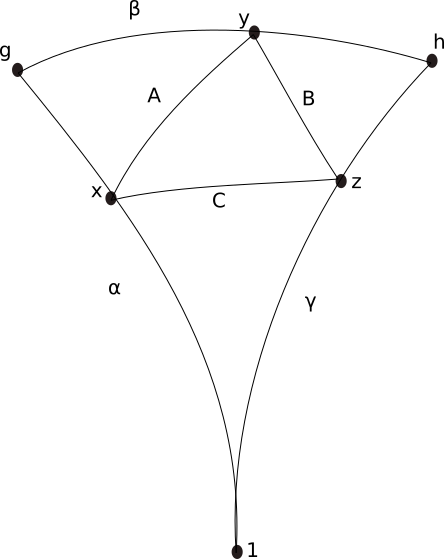
\includegraphics[scale=0.5]{treewidth.png}
		\caption*{}
	\end{figure}
	
	
	
	Ahora estamos listos para ver que $d(g,h) \le 3k$. Usamos la desigualdad triangular tres veces,
	\begin{align*}
		d(g,h) & \le d(g,x) + d(x,z) + d(h,z) \\
		& \le d(x,y) + d(x,z) + d(y,z) \le 3k
	\end{align*}
	tal como queríamos ver.
\end{proof}
	
	
\end{document}